\section{The Crust}
It is finally time to put the geometric tools that this paper has focused on so heavily to use to define the crust of a set of points. As a reminder, the crust is a method of curve reconstruction introduced by \cite{crust}, which is where all the definitions come from in this section. It begins with a set of points taken from a smooth curve with the assumption that they are close enough together to be reconstruction. This "close enough" condition is defined later in the section on sampling. The crust has the following simple definition:

\begin{definition}[The Crust]
	Let $S$ be a set of finite points in the plane, and let $V$ be the vertices of the Voronoi diagram of $S$. Next let $S'=S \cup V$ and consider the Delaunay Triangulation of $S'$. Any edge of the Delaunay triangulation of $S'$ that connects two points in $S$ is an edge of the crust.
\end{definition}

INSERT A FIGURE IN THIS SECTION WITH AN EXAMPLE SIMILAR TO PAGE 3 OF THE PAPER

This is a fairly simple definition, and yet I claim that it can often successfully reconstruct a curve from a set of points in the plane. Before formally proving that this is true for a certain sampling condition, I will provide some intuition on why this is the case. To do this, I will give an alternate but equivalent definition of the crust that uses the familiar empty circle property:

\begin{definition}[Alternate Definition of The Crust]
	Let $S$ be a set of finite points in the plane, and let $V$ be the vertices of the Voronoi diagram of $S$. An edge connecting two points in $S$ belongs to the crust of $S$ if there is a disk containing no other points in $S \cup V$.
\end{definition}

It also helps to note that Voronoi vertices are at the corners of regions of proximity, so they are closer to the points from $S$ in adjacent Voronoi regions than to any other points in $S$. This means that points that obey the alternative definition are connected with those in nearby proximity regions, not simply points that are closest together.

Also, looking at a few examples of Voronoi diagrams of many points, one can see that the diagram draws a line approximately through the middle of the shape that they create. This line is called the medial axis and will be explained further in the next section, but the idea is that the Voronoi edges trace out a line through the middle of a shape, then the empty circle properly serves to prevent lines from being drawn through this center line of the shape.

\subsection{The Medial Axis}

This section focuses on the medial axis, a tool that is used to define the conditions for sampling that guarantee that the crust can reconstruct a curve.
It is essentially a Voronoi diagram for a continuous curve, rather than a discrete set of points.
This becomes clear by the following definition that looks very similar to the alternate definition of the Voronoi diagram.


\begin{definition}[The Medial Axis]
	The medial axis of a smooth curve $F$ is the set of all points in the plane that are nearest to at least two points in $F$.
\end{definition}

\begin{figure}
	\centering
	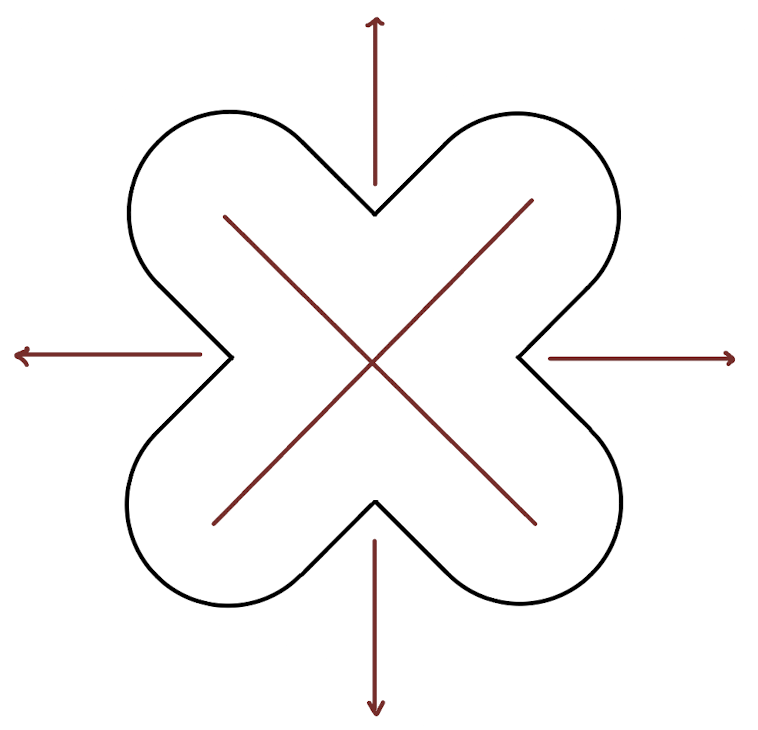
\includegraphics[width=0.6\linewidth]{figure_source/medial_axis_2.png}
	\caption{An example of the medial axis (gray lines) of a curve (black lines)}
	\label{fig:medial_axis}
\end{figure}


An example is shown in Figure~\ref{fig:medial_axis}, where the medial axis appears to be a sort of midline of the curve.

The following lemma will get us lots of mileage when proving results about the medial axis.

\begin{lemma}
	Any disk $B$ containing at least two points of a smooth curve $F$ either intersects $F$ in a single curve segment or contains a point of the medial axis (or both).
	\label{lem:single_curve_segment}
\end{lemma}

\begin{proof}
	If $B\cap F$ is a single curve segment, we are done.

	If the intersection contains a closed loop, then there is a medial axis internal to the loop which is inside $B$, so we are done.

	Otherwise, the intersection consists of two or more connected components $F$.
	Let $c$ be the center of $B$ and $p$ be the nearest point of $F$ to $c$.
	If there is more than one such $p$, $c$ is a point of the medial axis, and we are done.
	If not, consider $q$, the nearest point to $c$ on a different curve segment than $p$.
	Since $c$ is the center and $q\in B$, any point on $\overline{cq}$ is closer to $q$ than any point outside $B$.
	If we imagine walking along $\overline{cq}$, we start closest to $p$, and at some point cross over and are closer to $q$.
	At this point, we are nearest to both $p$ and $q$, so this point belongs to the medial axis, and we are done.
\end{proof}

And the next lemma allows us to connect Voronoi vertices to the medial axis, bridging our discrete geometric tools used to generate the crust with the continuous nature of a smooth curve and medial axis.


\begin{lemma}
	Any Voronoi disk $B$ of a finite set $S \subset F$, where $F$ is a smooth curve, must contain a point of the medial axis of $F$.
	\label{lem:voronoi_disk_contains_m}
\end{lemma}

\begin{proof}
	There are two cases:
	\begin{enumerate}
		\item{All samples are on the border of $B$ and no part of $F$ is inside.
		      In this case, the center of $B$ is a part of the medial axis.}
		\item{In the neighborhood of some sample $s$, $G=F-s$ intersects $B$. Here, there are three more cases:}
		      \begin{itemize}
			      \item{$G$ lies entirely on the edge of $B$. Here, the center of $B$ is part of the medial axis.}
			      \item{$G$ is entirely inside $B$. Here, there exists a smaller disk $B_\rho$ inside $B$ that does not intersect $G$ in a single curve segment, so lemma~\ref{lem:single_curve_segment} applies}
			      \item{$G$ crosses from outside to inside $B$ at $s$, then it must leave elsewhere creating a curve segment. Along with the other samples on the edge of $B$, $F\cap B$ is not a single curve segment, so lemma~\ref{lem:single_curve_segment} applies}
		      \end{itemize}
	\end{enumerate}
\end{proof}

\subsection{Sampling}

This section I provide an empirical definition of sampling, basically meaning how close together points are taken from a smooth curve.
Sampling is defined using a \textit{local feature size} function at any given point.
This function does what it says in the name, returning a number indicating how big features are at the point passed in.
So, if there is a large flat region, the local feature size will be large, and if there are tight turns, then it will be small.

\begin{definition}[Local Feature Size]
	The local feature size at some point $p$ on a smooth curve $F$, denoted $LFS(p)$, is the Euclidean distance from $p$ to the nearest point on the medial axis.
\end{definition}

If we think of the medial axis as a sort of midline, in a wide chasm, the medial axis will be very far from the edges, so the local feature size will be large.
On the other hand, through a winding tunnel, the midline is very close to either edge, so the local feature size is very small.

Now we can define a sampling condition, which is just a proportionality factor of our local feature size.

\begin{definition}[r-sampled Curve]
	A smooth curve $F$ is r-sampled by a set of points $S$ if every $p\in F$ is within distance $r\cdot LFS(p)$ of a sample $s\in S$.
\end{definition}

And now we reach our last couple definitions describing disks that and points lie between two sample points.

\begin{definition}[Curve Voronoi Disk and Vertex]
	A curve Voronoi disk is a maximal disk, empty of sample points that is centered at a point on a smooth curve. The point on the curve is the curve Voronoi vertex.
\end{definition}

We are finally equipped to start proving that the crust really will reconstruct a curve under the proper conditions.
Before beginning these proofs, we should note that
The first step on this path is to prove that a curve Voronoi disk always intersects the curve in a single curve segment.

\begin{lemma}
	A curve Voronoi disk, $B$, intersects an r-sampled curve $F$ in a single curve segment if $r\le 1$.
	\label{lem:curve_voronoi_single_curve_segment}
\end{lemma}

\begin{proof}
	Consider the contrapositive: If $B$ does not intersect $F$ in a single curve segment then $r > 1$.
	If this assumption is true, there must a point of the medial axis inside $B$ by lemma~\ref{lem:single_curve_segment}.
	In this case, the radius of $B$ must be greater than $LFS(p)$.
	And since the maximum radius of a curve Voronoi disk is the distance from $p$ to the nearest sample point, which is $r\cdot LFS(p)$, the only way for a curve Voronoi disk to have radius greater than the local feature size is if $r > 1$.
\end{proof}

And moreover,

\begin{lemma}
	Let $F$ be an r-sampled curve with $r \le 1$. There is a curve Voronoi disk connecting each pair of adjacent samples.
	\label{lem:cruve_voronoi_disk_connects}
\end{lemma}

\begin{proof}
	Let $s_1$ and $s_2$ be adjacent samples along $F$.
	The curve segment between $s_1$ and $s_2$ intersects the bisector of $\overline{s_1s_2}$ at least once.
	Let $p$ be a curve Voronoi vertex at one of these intersections.
	If the corresponding curve Voronoi disk, $B$, has both samples on its boundary, we are done.
	Otherwise, there exists some sample $s$ closer to $p$ than both $s_1$ and $s_2$ on some other part of $F$.
	If this is true, then $B$ does not intersect $F$ in a single curve segment, thus violating lemma~\ref{lem:curve_voronoi_single_curve_segment}, so no such $s$ exists.
\end{proof}

This happens to be very similar to the empty circle property used to define the Delaunay triangulation.
So similar, in fact, that we can make the following statement:

\begin{theorem}
	Let $F$ be an r-sampled smooth curve in the plane, $r < 1$.
	The Delaunay triangulation of the set $S$ of samples contains an edge between every adjacent pair of samples.
\end{theorem}

\begin{proof}
	For any triangle in the Delaunay triangulation, you can resize the circumcircle so that it connects any pair of points in the triangle at all possible center points.
	Do this for every triangle, and you have a collection of all circles that connect two adjacent samples.
	Obviously, each curve Voronoi disk must be in this collection of circles.
\end{proof}

This theorem should provide some confidence that the crust can actually reconstruct a curve, but there is still much work to be done to prove this result.

\subsection{Curvature}

Next, we turn to getting a concrete lower bound for how large the angle between points on a curve can be given the sampling conditions.
In other words, we will show that there is a limit to how much a smooth curve $F$ can bend given $r$.
The idea here is to find a disk that is tangent to $F$ that does not have any points in its interior, then say that the maximum curvature is along its edge.
One such circle tangent to any $p\in F$ is a circle of radius $LFS(p)$.

\begin{lemma}
	A disk tangent to a smooth curve $F$ at a point $p\in F$ with radius at most $LFS(p)$ contains no points of $F$ in its interior.
	\label{lem:tangent_disk}
\end{lemma}

\begin{proof}
	The largest empty disk tangent to $p$ has a center point $m'$.
	Since this disk is maximal, there must be at least one other point on its boundary.
	This means that there is more than one nearest point to $m'$, so $m'$ belongs to the medial axis.
	So, the radius of the disk is at most $LFS(p)$.
\end{proof}

\begin{figure}
	\centering
	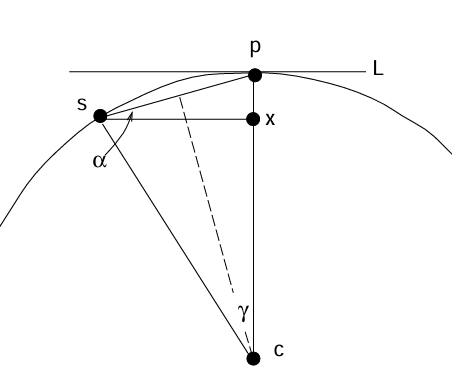
\includegraphics[width=0.6\linewidth]{figure_source/tangent_circle_properties.png}
	\caption{TEMPORARY -- copied from paper, Line L is tangent to the circle at p, and the distance between c and p and c and s is L, and the distance from s to p is $L\cdot r$}
	\label{fig:tangent_circle_properties}
\end{figure}


Now let's view some properties for such a circle.
In Figure~\ref{fig:tangent_circle_properties}, $c$ is the center point, so label the radii $LFS$ for the local feature size
Next, label the distance from $s$ to $p$ as $LFS\cdot r$ to represent that this $s$ is the closest point allowed to $p$ given that the curve is r-sampled.
Now note the following properties:
\begin{itemize}
	\item{The length of $\overline{sx}$ is $LFS\cdot \sin \gamma$ }
	\item{The distance between s and p, $LFS\cdot r = 2LFS\cdot\sin (\frac{\gamma}{2})$, so $\gamma = 2 \arcsin (\frac{r}{2}) $}
	\item{$\alpha = \frac{\gamma}{2} = \arcsin (\frac{r}{2})$ }
	\item{The angle between $L$ and $p$ and $\overline{sp}$ is $\alpha$}
\end{itemize}

Now we are ready to derive a lower bound on the curvature:
\begin{lemma}
	For an r-sampled curve, $r < 1$, the angle formed at a curve Voronoi vertex between two adjacent samples is at least $\pi - 2\arcsin(\frac{r}{2})$.
\end{lemma}

\begin{proof}
	By lemma~\ref{lem:tangent_disk}, there can be no points of the curve inside a disk of radius $LFS(p)$ tangent to the curve.
	So, the tightest curve can be along the edge of the disk.
	In this case, the point labeled p in Figure~\ref{fig:tangent_circle_properties} is in exactly this configuration.
	And from the figure it is clear that the triangle formed by $p$ and two samples is isoscles with the duplicate angle equal to $\alpha$.
	So, the angle formed at $p=\pi-2\alpha = \pi-2\arcsin(\frac{r}{2})$ by the properties listed above.
\end{proof}

And following closely from that,

\begin{lemma}
	For an r-sampled curve, $r < 1$, the spanned by three adjacent samples is at least $\pi - 2\arcsin(\frac{r}{2})$.
\end{lemma}

\begin{proof}
	Begin with the case of the curve Voronoi vertex with a corresponding central angle $2\gamma$.
	The angle at $p$ is an inscribed angle which is half of the central angle $2\pi - 2\gamma$.
	Now to add a third sample, just place another curve Voronoi vertex next to one of samples, then another sample next to that.
	Now there are two places with central angle $2\gamma$, so the total central angle is doubled.
	This makes the corresponding inscribed angle, now at the middle sample, half of $2\pi - 4\gamma = \pi - 4\arcsin(\frac{r}{2})$
\end{proof}

For lack of a better term, these results show that if you zoom in on any three samples from $F$, the curve appears pretty flat.
As an example, for $r = 0.5$, the largest angle between any three sample points is just above $122^\circ$.

\subsection{Guaranteeing Reconstruction}

Finally, we have the background to provide an upper bound on $r$ so that an r-sampled curve will \textit{always} be reconstructed by the crust.
To prove that a curve is reconstructed, we need to prove that all adjacent edges are included in the crust and that no other edges are.
I will provide this bound separately for each of these requirements, and the lower of the two will be an upper bound that guarantees the crust successfully reconstructs the curve.
The idea behind each of these proofs is that I will be making the minimum assumptions required on r to give the mere possibility that the crust does not reconstruct the curve, then at the end I will flip the inequality on $r$, so this possibility does not exist.

\begin{theorem}
	The crust of an r-sampled curve with $r < 0.40$ contains an edge between every pair of adjacent vertices.
\end{theorem}

\begin{proof}
	An edge appears in the crust if and only if there is a circle connecting its vertices empty of other sample points and Voronoi vertices.
	By Lemma~\ref{lem:cruve_voronoi_disk_connects}, we know that there is a curve Voronoi disk, $B$, touching each pair of adjacent vertices.
	So, $B$ fits the condition to have its samples form an edge in the crust if it is also empty of Voronoi vertices.

	So, I will provide a lower bound on $r$ that \textit{could} allow there to be a Voronoi vertex in $B$, then flip this bound to ensure it cannot exist.

	Let the midpoint of $B$ be called $p$.
	We know that the radius of $B$ is at least $r\cdot LFS(p)$, by definition of r-sampled.
	Let Voronoi vertex $v$ live inside $B$, with a corresponding Voronoi circle $V$ with radius $R$, the distance to the nearest sample point on the boundary of $B$.
	Note that $R$ is maximized when it is on the boundary of $B$, a distance $r\cdot LFS(p)$ from $p$.
	By lemma~\ref{lem:voronoi_disk_contains_m}, $V$ must contain some point of the medial axis.

	Now, by the definition of local feature size, the disk, $B'$, of radius $LFS(p)$ centered at $p$ cannot contain a point in the medial axis.
	So, all there is to do is choose $r$ so that some part of $V$ is not inside $B'$, so there is no guarantee that a point in the medial axis is inside $B'$.
	In other words, we need $r\cdot LFS(p) + R > LFS(p)$.

	Let us now maximize $R$.
	We know that the angle between $p$ and the two samples on the boundary of $B$ is at least $\pi - 2\arcsin(\frac{r}{2})$ by the properties from Figure~\ref{fig:tangent_circle_properties}.
	Or on the other side, it is at most $2\pi$ minus this angle, $2\pi - (\pi - 2\arcsin(\frac{r}{2})) = \pi + 2\arcsin(\frac{r}{2})$.
	Let $v$ be on this side so that it is as far as possible from the sample points.
	The furthest that $v$ can be from either sample point is when it is at half this angle around the circle, at a maximum angle of $\frac{1}{2} (\pi + 2\arcsin(\frac{r}{2}))$, call this angle $\psi$.
	Clearly, $\frac{R}{2} \le r \cdot LFS(p) \sin (\frac{\psi}{2})$, so finally:

	\[
		r\cdot LFS(p)+2r\cdot LFS(p)\sin \left(
		\bigfrac{\pi + 2\arcsin(\frac{r}{2})}{4}
		\right)
		>
		LFS(p)
	\]
	or
	\[
		r+2r\sin \left(
		\bigfrac{\pi + 2\arcsin(\frac{r}{2})}{4}
		\right)
		>
		1
	\]

	It is easy to verify that the inequality is satisfied for $r > 0.40$, so we flip the inequality to guarantee that no such situation can occur to get $r \le 0.40$
\end{proof}

\begin{theorem}
	The crust of an r-sampled smooth curve does not contain any edge between non-adjacent vertices for r < 0.252
\end{theorem}






